\chapter[Corporate tax revenues in OECD countries]{Corporate tax revenues\\in OECD countries}
\vspace{-10pt}
So far, it has been described how governments are influenced in setting their corporate tax rates as part of a strategic game with other countries. Over time, the relaxation of capital controls has increased tax competition between states, ultimately resulting in lower statutory tax rates. That said, I have wondered about the effects of such a sharp reduction in tax rates on governments' tax revenues.  This second paper, titled "Corporate tax revenues in OECD countries" by \textcite{clausing}, investigates tax revenue trends by breaking down their components.

\section{The elements that build up tax revenues}

In an international context with downward pressure on tax rates, the author's ultimate goal is to make policymakers aware of the determinants of tax revenues. Indeed, tax revenues are certainly determined by tax rates, but not only, and \textcite{clausing} builds them, in GDP terms, as a function of:
\begin{equation}\label{eq3.1}
    \frac{CorporateTaxRevenue}{GDP}=T\times f\times \Pi \times CS
\end{equation}
where $T$ is the statutory tax rate $T=\frac{TaxesDue}{TaxBase}$, $f$ is the extent of the tax base $f=\frac{TaxBase}{CorporateProfits}$, $\Pi$ is the profitability of firms $\Pi=\frac{CorporateProfits}{CorporateValueAdded}$, and $CS$ their size in the economy $CS=\frac{CorporateValueAdded}{GDP}$. Later in the empirical analysis, this simple model will be expanded with other key components, such as the structure of the tax system, international interactions and the size of the country, which may also have an effect on fiscal revenues.

By deriving Eq. \ref{eq3.1} for $T$ and taking advantage of the chain rule, it can be generalized the effect of a change in the statutory tax rate on the corporate tax revenues of the state:
\vspace{-10pt}
\begin{equation}\label{eq3.2}
\scalemath{0.85}{
    \frac{\partial Revenue}{\partial T}=\underbrace{f\times \Pi \times CS}_{(1)}+\underbrace{T\times \frac{\partial f}{\partial T}\times \Pi \times CS}_{(2)}+\underbrace{T\times f\times \frac{\partial \Pi}{\partial T} \times CS}_{(3)}+\underbrace{T\times f\times \Pi \times \frac{\partial CS}{\partial T}}_{(4)}}
\end{equation}
where the first term represents the marginal increase in revenues due to the higher $T$, however, firms behave to increased tax rates, and the following terms describe their behaviour. The second term captures firms' efforts to reduce their tax base. The third deals with firms' profits and, for instance, may capture a decrease in taxable profits caused by a shift of profits to countries with lower tax rates. The last term relates to firms' participation in the economy, and, for example, a high tax rate may cause a firm to relocate or reduce its production, ultimately shrinking its contribution to national GDP. To sum up, the last three terms represent the tax avoidance efforts a company may undertake subsequently a tax increase. However, \textcite{clausing} suggests that the overall effect of Eq. \ref{eq3.2} is ambiguous, because, ultimately, the outcome depends both on the size of the direct effect, first term, and on the strength of the firms' tax avoidance activities.

\section{Testing the theory}

\subsection{An empirical model}

So far, \textcite{clausing} decomposes the components of tax revenues, and emphasises the consequences of a tax rise on firms' behaviour. A company may respond by changing its long-term strategy or by initiating tax avoidance and, at the extreme, evasion practices.

To empirically estimate the effects of all the components just described on tax revenues, the author constructs the following regression equation:
\begin{align}\label{eq3.3}
    \left( \frac{CorporateTaxRevenue}{GDP}\right)_{it}=\alpha &+\beta_1 TaxRate_{it}\notag \\
    &+\beta_2 TaxRate^2_{it}\notag \\
    &+\beta_3 CorporateProfitability_{it}\notag \\
    &+\beta_4 SizeCorporateSector_{it}
\end{align}
Eq. \ref{eq3.3} mirrors Eq. \ref{eq3.1} with two additional adjustments.  Firstly, as in \textcite{dev-loc-red-08}, where the authors do not find an unambiguous measure for the EMTR, ultimately using a measure for effective tax wedge, likewise \textcite{clausing} decides to omit the variable about the tax base, $f$, in the regression equation, Eq. \ref{eq3.3}. On the other hand, an extra variable, $TaxRate^2_{it}$, is included, whose intent is to capture any nonlinear effects between tax rate and tax revenues.

\subsection{Data}

To estimate the coefficients of Eq. \ref{eq3.3}, \textcite{clausing} uses panel data from 29 OECD countries between 1979 and 2002. This paper handles very similar data to the previous article of \textcite{dev-loc-red-08}, helping us build an analysis~with~similar~basis. Certainly, both also chose OECD data because of its high availability and reliability~too.

\begin{figure}[!h]
    \centering
    \captionsetup{font=footnotesize}\caption{time series for avg. statutory tax rate and corporate income rev./GDP, \cite{clausing}}
    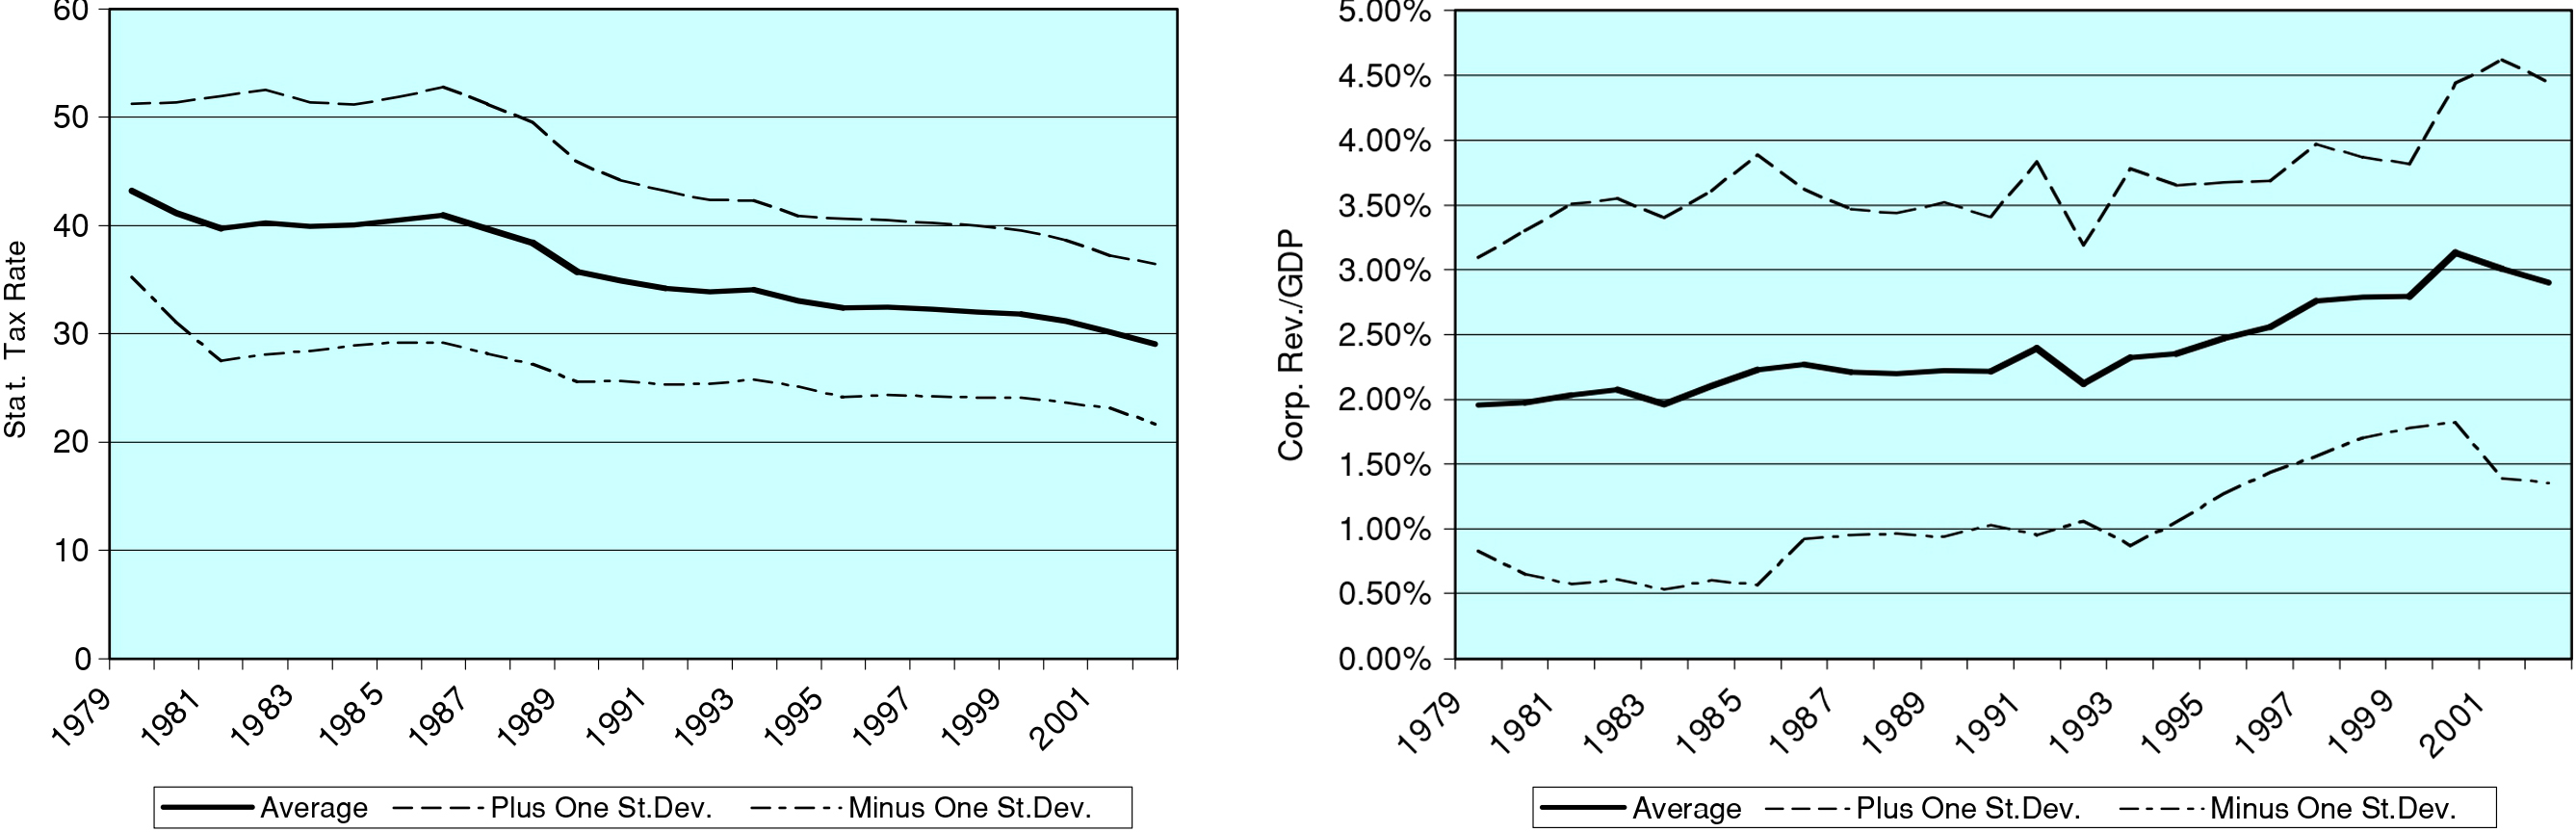
\includegraphics[width=.85\textwidth]{img/clausing-trends.jpg}
    \label{clausing-img}
    \vspace{-5pt}
\end{figure}
Before delving into the regression results, let us illustrate the context from which the data used for the regression comes. On the left, Figure \ref{clausing-img} shows the trend for the average statutory tax rate over the 24 years time frame. Similarly to \textcite{dev-loc-red-08}, also here is clear the downward movement of the tax rate, specifically from almost 45\% in 1979 to slightly below 30\% in 2002.  On the right side, Figure \ref{clausing-img} represents the average corporate tax revenues (in GDP terms) over the years. Interestingly and almost counterintuitively, although the fall of the tax rates set by the governments, the average of the fiscal revenues grows over time, from 2\% in 1979 to almost 3\% in 2002. This outcome may come from a series of factors. Firstly, \textcite{clausing} reports that the closest data on corporate profitability of firms over the period examined increased from 33\% to 39\%. Secondly and more importantly, the states increased their tax base over this time frame. This assumption is also supported by another article by Michael P. Devereux, specifically \textcite{dev-2002}. There, the authors examine data from 16 OECD countries between 1982 and 2001, taking governments' tax base broadening reforms as a given.
\vspace{-5pt}
\section{Empirical results}

In Table \ref{tab:clau-1}, the estimated coefficients for Eq. \ref{eq3.3} are displayed.
\begin{table}[ht]
\centering
\captionsetup{font=small}\caption{regression results, \textcite{clausing}}
\scalebox{0.9}{
\begin{tabular}{llll}
\hline
 & (1) & (2) & (3)\\
\hline
Tax     & 0.147             & 0.186             & 0.154\\
        & (0.022)$^{**}$    & (0.025)$^{**}$    & (0.026)$^{**}$\\
Tax$^2$    & -0.221            & -0.236            & -0.185\\
        & (0.039)$^{**}$    & (0.051)$^{**}$    & (0.052)$^{**}$\\
Profit rate &               & 0.106             & 0.105\\
            &               & (0.014)$^{**}$    & (0.013)$^{**}$\\
Corp. share &               & 0.053             & 0.042\\
            &               & (0.011)$^{**}$    & (0.009)$^{**}$ \\
Credit      &               &                   & 0.005\\
            &               &                   & (0.002)$^{**}$\\
Mixed       &               &                   & -0.000\\
            &               &                   & (0.001)\\
Constant    & 0.002         & -0.077            & -0.067\\
            & (0.003)       & (0.011)$^{**}$    & (0.009)$^{**}$\\
Observations & 587 & 282 & 282\\
R-squared & 0.13 & 0.43 & 0.46\\
\hline
\end{tabular}}
\label{tab:clau-1}
\vspace{-2pt}
\end{table}
In all three specifications, the statutory tax rate plays the biggest role. An increase in the tax rate is correlated to an increase in tax revenues/GDP between $0.147$ and $0.186$. Moreover, with the estimated coefficient for the tax rate in Equation (1), \textcite{clausing} is able to estimate the hypothetical revenues/GDP for every tax rate. Plotting it on a graph becomes very intriguing, as the left side of Figure \ref{clausing-img-2} reveals that this relationship is parabolic and the tax rate that maximizes tax revenue/GDP would be about 33\%. In any case, this value is not to be read as optimal, neither for the government nor the households, since it is derived from hypothetical revenues. However, it would be a curious exercise for jurisdictions to find their profit-maximizing tax rate, compare it with the current one, and see if there is room for improvement, with the ultimate goal of having a larger fiscal budget and being able to better provide public goods and address social problems.
\begin{figure}[!h]
    \centering
    \captionsetup{font=small}\caption{estimated revenue-tax curves, \cite{clausing}}
    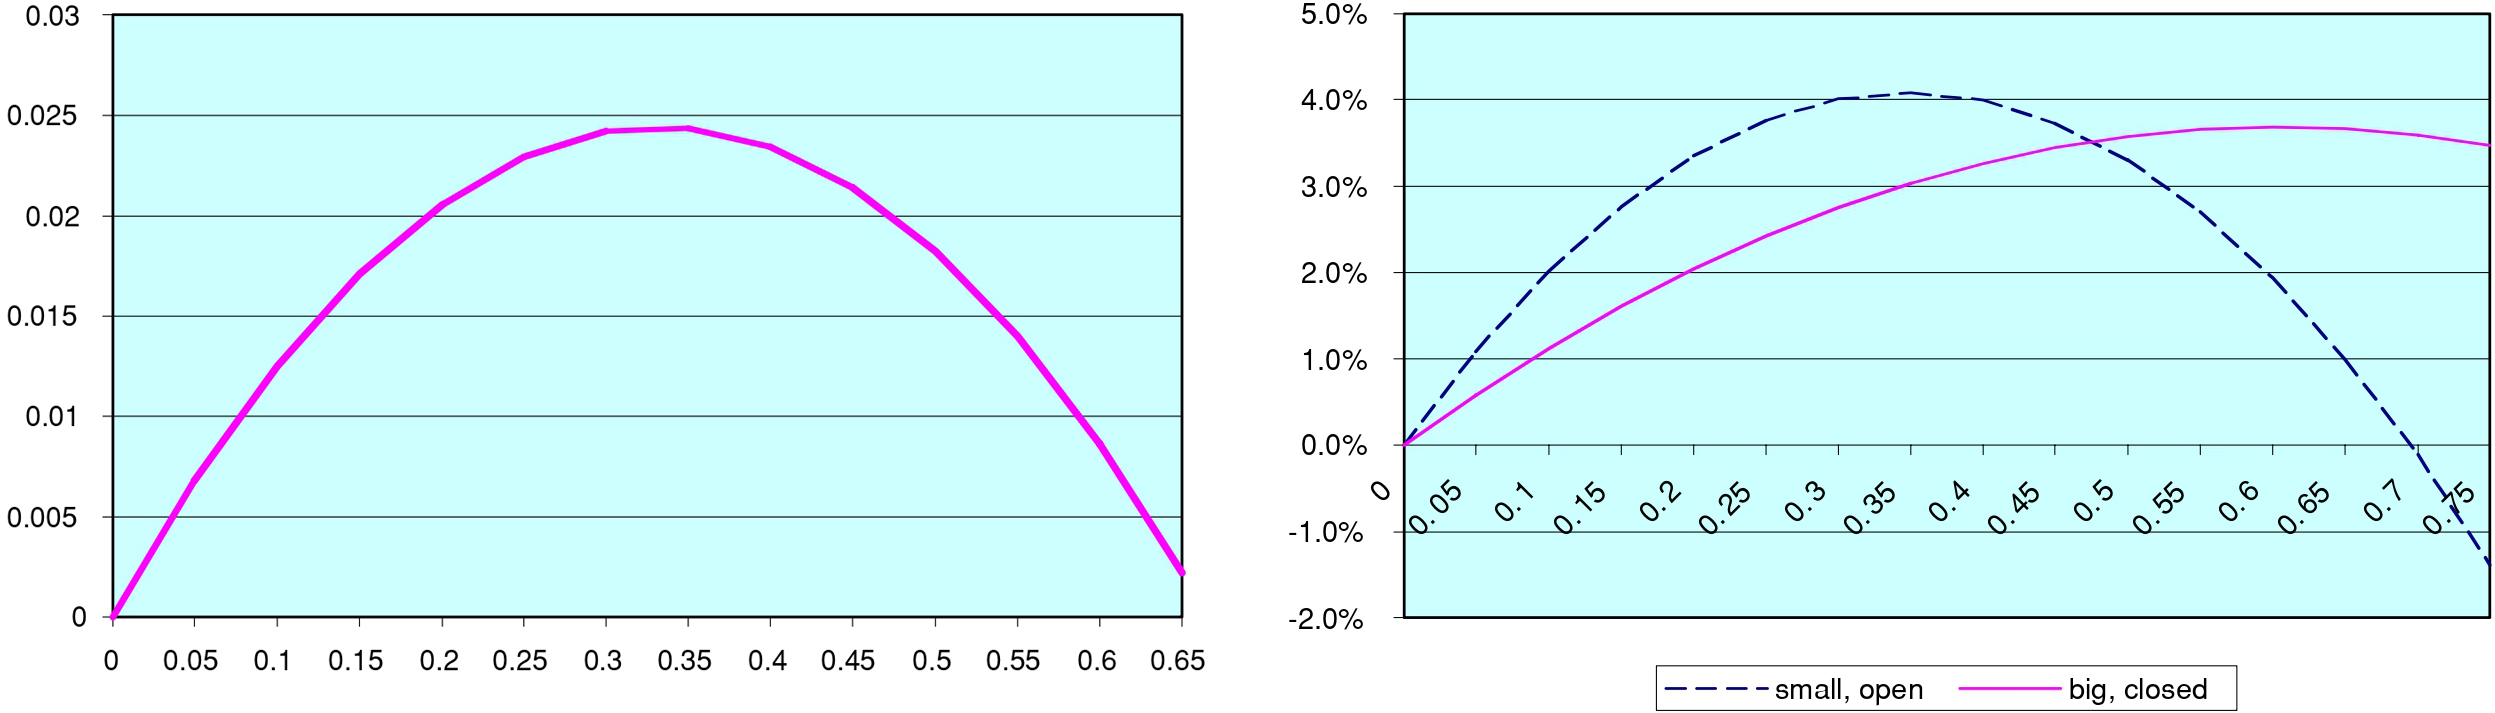
\includegraphics[width=.85\textwidth]{img/clausing-rev-max.jpg}
    \label{clausing-img-2}
    \vspace{-2pt}
\end{figure}

In Table \ref{tab:clau-1}, Equation (2) includes two more regressors: corporate profitability and the size of the corporate sector. The estimated coefficient about the firms' profits, $\beta_3$, appears to have a relevant force towards higher tax revenues. Intuitively, the higher the firms' profits, and therefore the taxable income, the higher the government's revenues. Finally, Equation (3) once again extends the regression by including two dummy variables on the structure of the tax system, depending on whether the country has in place a credit or mixed (credit and territorial) tax system. Although the economic significance may not be substantial, the effect of the dummy variable on credit systems is statistically significant and implies that countries that allow tax credits on taxes paid abroad on foreign incomes can expect a 5\% increase in their revenues/GDP. The limited economic relevance of this outcome confirms why, nowadays, most jurisdictions adopt a territorial system. As a matter of fact, the main problem of a tax credit system is that foreign income is taxed locally only when it is repatriated.  To overcome this problem, governments have preferred the territorial system while strengthening international tax coordination.

\begin{table}[t]
\centering
\captionsetup{font=small}\caption{regression results for extended equations, \textcite{clausing}}
\scalebox{0.9}{
\begin{tabular}{lllll}
\hline
& (1) & (2) & (3)\\
\hline
Tax                                 & 0.133            &  0.214                & 0.182 \\
                                   & (0.020)$^{**}$    &  (0.026)$^{**}$                 & (0.026)$^{**}$ \\
Tax$^2$                             & -0.156            &  -0.320                & 0.250 \\
                                   & (0.035)$^{**}$    & (0.045)$^{**}$                  & (0.047)$^{**}$ \\
\dots & \dots & \dots & \dots \\
Intl * tax                         & 0.053             &                   & 0.055 \\
                                   & (0.018)$^{**}$    &                   & (0.017)$^{**}$ \\
Intl * tax$^2$                     & -0.088            &                   & -0.096 \\
                                   & (0.044)$^{*}$     &                   & (0.041)$^{*}$ \\
Big * tax                          &                   & -0.060            & -0.054 \\
                                   &                   & (0.016)$^{**}$ & (0.016)$^{**}$ \\
Big * tax$^2$                      &                   & 0.149 & 0.137 \\
                                   &                   & (0.040)$^{**}$ & (0.038) \\
Constant                    & -0.026            & -0.039 & -0.031 \\
                    & (0.010)$^{*}$     & (0.011)$^{**}$ & (0.011)$^{**}$ \\
Observations & 513 & 513 & 513 \\
R-squared & 0.27 & 0.23 & 0.28\\
\hline
    \end{tabular}}
    \label{tab:clau-2}
    \vspace{-2pt}
\end{table}

Before concluding the analysis, \textcite{clausing} extends one more time the regression, and two additions are noteworthy. In Table \ref{tab:clau-2}, equations are all built on Equation (3) of Table \ref{tab:clau-1}, and here, for the sake of readability, only part of the regressors are listed. First, in Equation (1), two terms interact: the tax rate and a dummy variable, $international$, taking value one if the country is particularly open to trade, meaning that its FDI relative to GDP are above average. The regression captures that more open economies face a steeper revenues-tax rates curve and, therefore, higher tax revenues from a tax increase. Second, Equation (2) includes another interaction term between the size of the country and the tax rate. The dummy variable $big$ is set to one if the country's population size is above average. Assume bigger countries deal with less elastic capital, and conversely, smaller countries, the negative estimated coefficient confirms that large countries have a less steep revenue curve.

Using together the controls of Equations (1) and (2) gives Equation (3). Here, the last curious result confirms the previous outcomes, in other words, bigger and more close economies have a less steep revenue curve than smaller and opener ones. Conversely, small and open countries, at low tax rates, can obtain higher revenue gains from a tax rise than their larger counterparts. The two revenue curves of both kinds of countries can be seen on the right side of Figure \ref{clausing-img-2}. From this last result, countries can form their expectations on changes in revenues when adjusting their tax policies. If smaller and more open countries can be more ambitious in their revenue targets at low tax levels, the same cannot be said for their opposite, which must carefully touch rates, particularly if it needs to maintain a stable budget in the short term.